\documentclass[10pt]{beamer}

\mode<presentation> {
\usetheme{PaloAlto}
\setbeamercovered{transparent}
}

\setbeamertemplate{navigation symbols}{}
\setbeamercolor{Feather}{fg=black!20,bg=blue!50}
\setbeamercolor{structure}{fg=black}

\usepackage[utf8]{inputenc}
\usepackage[english]{babel}
\usepackage[T1]{fontenc}
\usepackage{helvet}
\usepackage{amsmath,amssymb,amsfonts}
\usepackage{hyperref} % Adds support for hyperlinks
\usepackage{physics}
\usepackage{framed, color}
\usepackage{epsfig}
\usepackage{acronym}
\usepackage{multirow, array}
\usepackage{float}
\usepackage{natbib}
\usepackage{fancyhdr}
\usepackage{xcolor}
\usepackage{multicol}
\usepackage{mdframed}
\usepackage{endnotes}
\usepackage{listings}
\usepackage{tensor}
\usepackage{csquotes}
\usepackage{tikz}

\setbeamercolor{structure}{fg=blue}
\setbeamercolor{title}{fg=blue!80!black}
\setbeamercolor{frametitle}{fg=blue!80!black, bg=blue!20}

\title[Progress]{\color{white}{\Large Project Progress}}

\author[Carlos Padilla,]{\normalsize Carlos Padilla} %Cesar Alejandro Perez Trinidad, Marlene Villanueva Tlatempa, Sebastian Vargas Hernández\\ \texttt{enigmak9@protonmail.com}}
\institute[]{\small ICN, UNAM}
\date{\today}
\logo{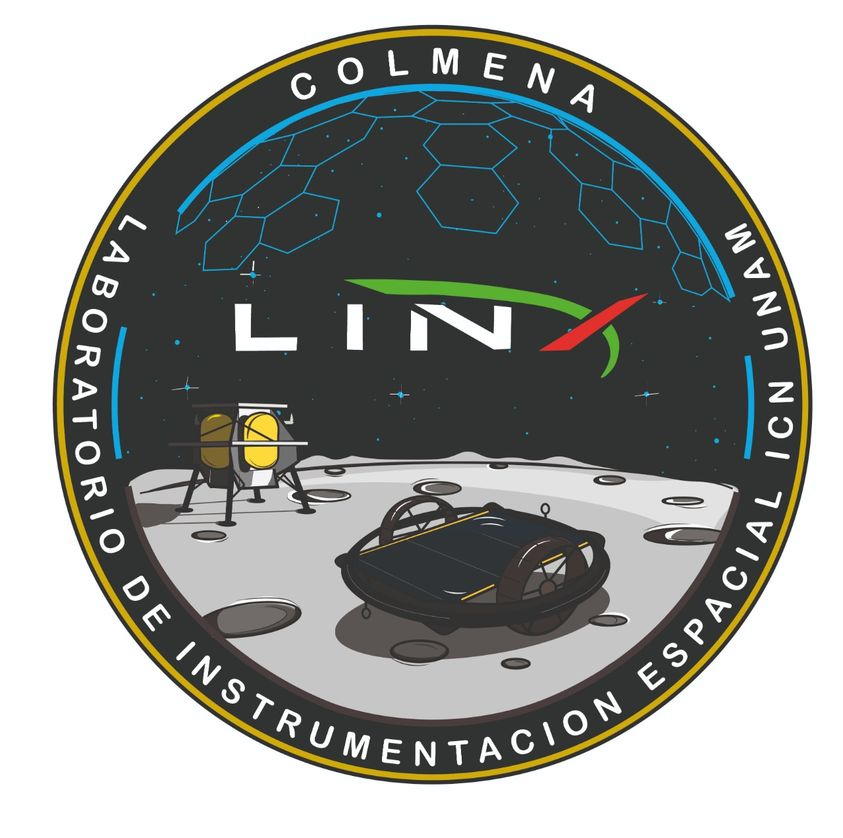
\includegraphics[height=1cm]{logo_linx.png}} % Adjust the height as needed

\begin{document}
\maketitle

%%\section{Bellman's equation}
%\begin{frame}
  %\frametitle{Bellman's equation}
  %\begin{equation%}
    %V(s) = \max_a \left\{ R(s, a) + \gamma V(s') \right\}
  %\end{equation}
  %\vfill
  %\centering
  %\hyperlink{https://www.overleaf.com/project/6612ccd97e0cee07ec75b8e1}{\beamergotobutton{Overleaf Project Link}}
%\end{frame}

\begin{frame}
  \frametitle{Task Execution Model}
  \centering
  \scalebox{1.8}{%
    \href{https://www.overleaf.com/project/6612ccd97e0cee07ec75b8e1}{%
      \[
        M_j = \left[I, t_j', \Delta t_j, P_{j}^{R}, P_{j}^{D}\right], \left[W_{I}^{R}, W_{I}^{D}\right]
      \]
    }
  }
  \vfill
  \centering
\end{frame}

\begin{frame}{Reward Function - Part 1}
  \href{https://www.overleaf.com/4694553851qmxvfhgchkkd#eea74e}{
  \begin{equation*}
    \xi_j = S_j P_j e^{\left(\frac{t_{j}^{E}-t_{j}^{R}}{\sigma}\right)^2} P_j^D d_j g(k)
  \end{equation*}}
\end{frame}

\section{Overall Performance Metric}

\begin{frame}
  \frametitle{Overall Performance Metric}
  \href{https://www.overleaf.com/4694553851qmxvfhgchkkd#eea74e}{
  \begin{equation*}
    \mathcal{\xi} = \sum_{j=1}^{J} \mathcal{\xi}_j + \frac{\alpha}{N} \sum_{i=1}^{N} \left( \frac{E_i - E_L}{E_{max} - E_L} \right)
  \end{equation*}}
\end{frame}

\section{Sample Data}
\begin{frame}{Sample Data}
  \href{https://github.com/EnigmaK9/linx/tree/main/06-progress_04_22_2024/padilla-villanueva/sql}{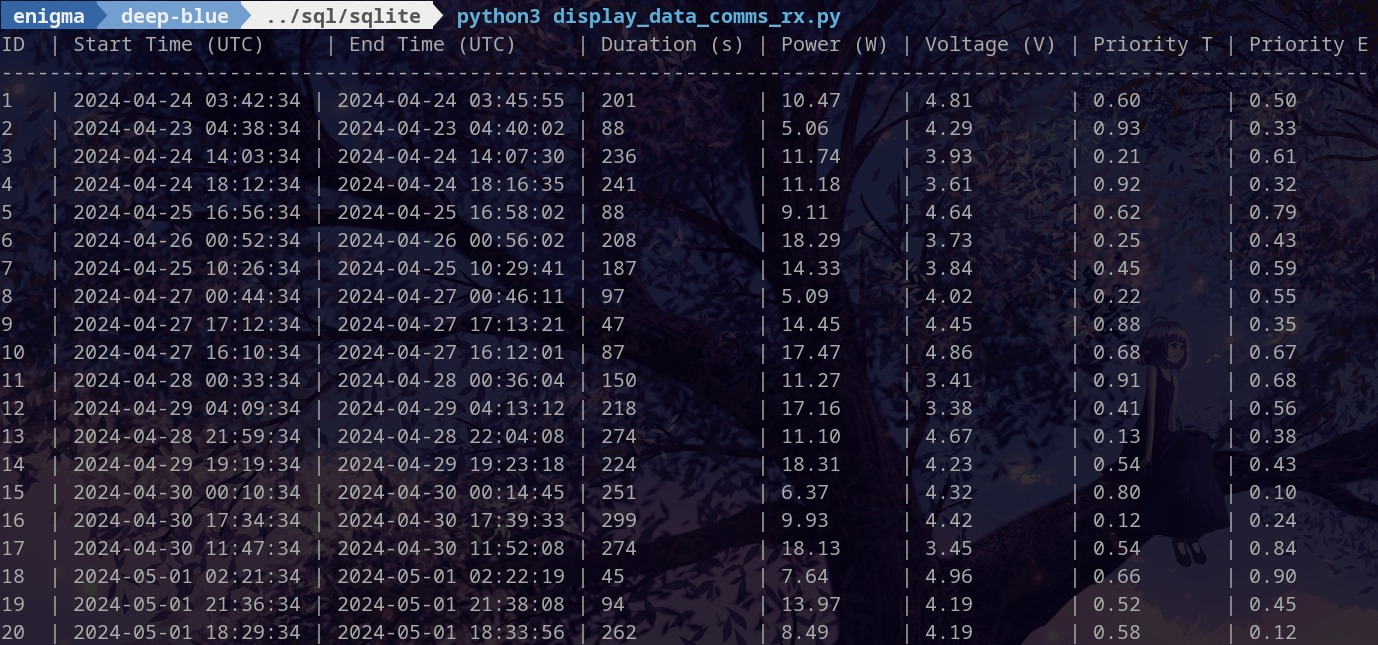
\includegraphics[width=0.9\textwidth]{sample_data.jpeg}}

\end{frame}

\section{Sample Data: OBC}
\begin{frame}{Sample Data: OBC}
  \href{https://github.com/EnigmaK9/linx/tree/main/06-progress_04_22_2024/padilla-villanueva/sql}{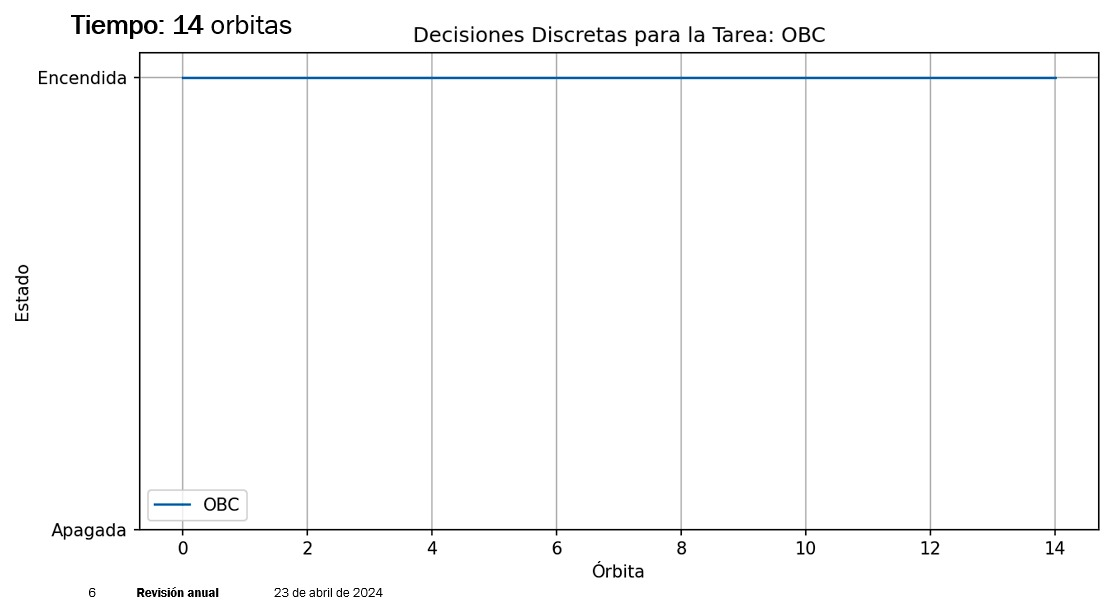
\includegraphics[width=0.9\textwidth]{obc.jpeg}}

\end{frame}

\section{Sample Data: Particle Detector}
\begin{frame}{Sample Data: Particle Detector}
  \href{https://github.com/EnigmaK9/linx/tree/main/06-progress_04_22_2024/padilla-villanueva/sql}{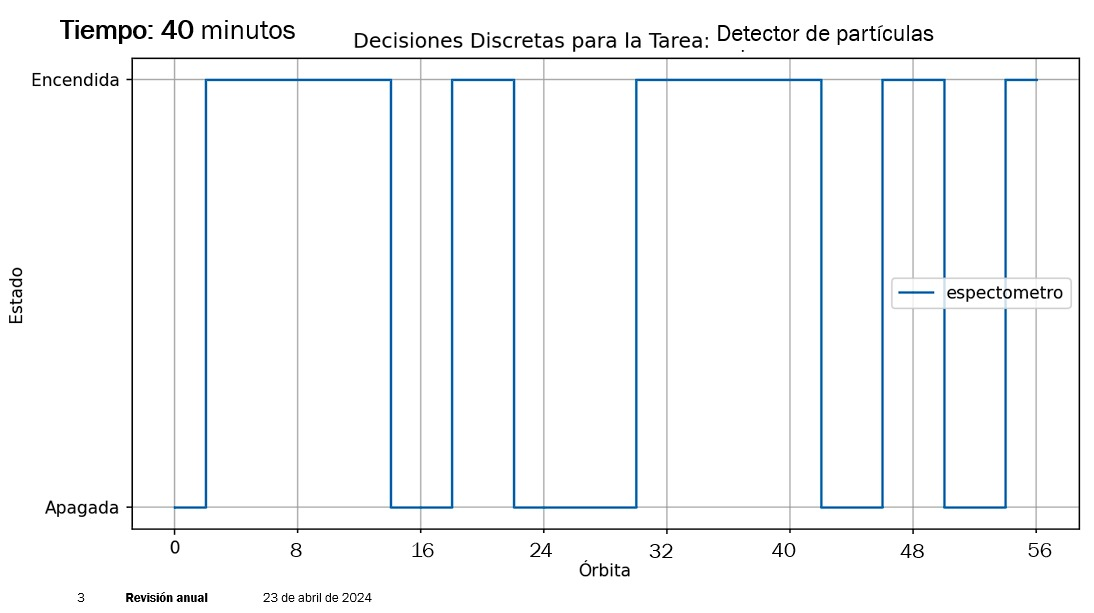
\includegraphics[width=0.9\textwidth]{detector.jpeg}}

\end{frame}

\section{Sample Data: Cámara}
\begin{frame}{Sample Data: Camera}
  \href{https://github.com/EnigmaK9/linx/tree/main/06-progress_04_22_2024/padilla-villanueva/sql}{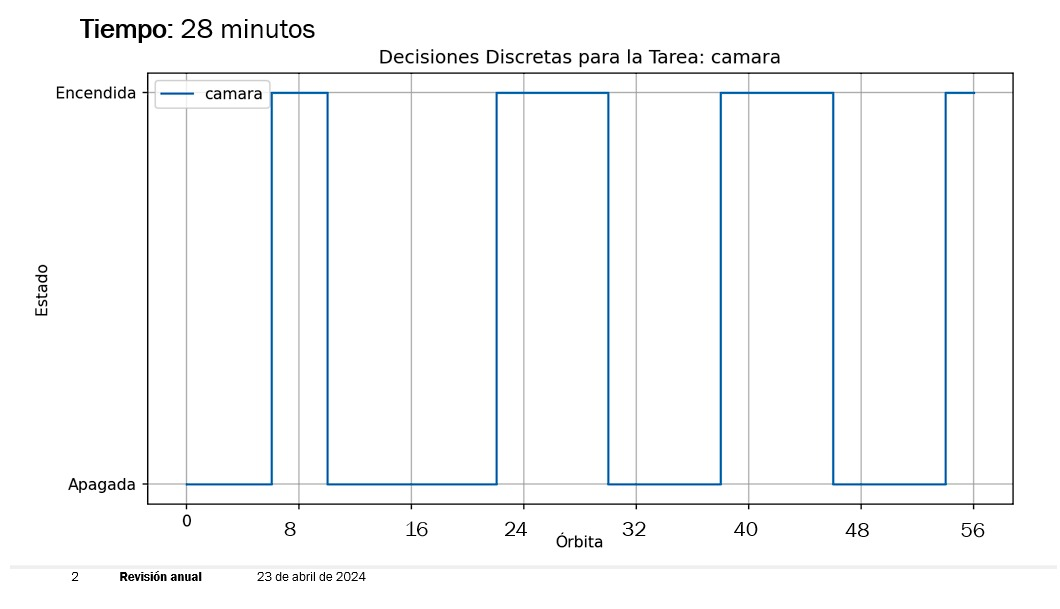
\includegraphics[width=0.9\textwidth]{camara.jpeg}}

\end{frame}

\section{Data upload}
\begin{frame}
  \frametitle{Data upload}
  \centering
  \href{https://github.com/EnigmaK9/linx/tree/main/06-progress_04_22_2024/padilla-villanueva/sql}{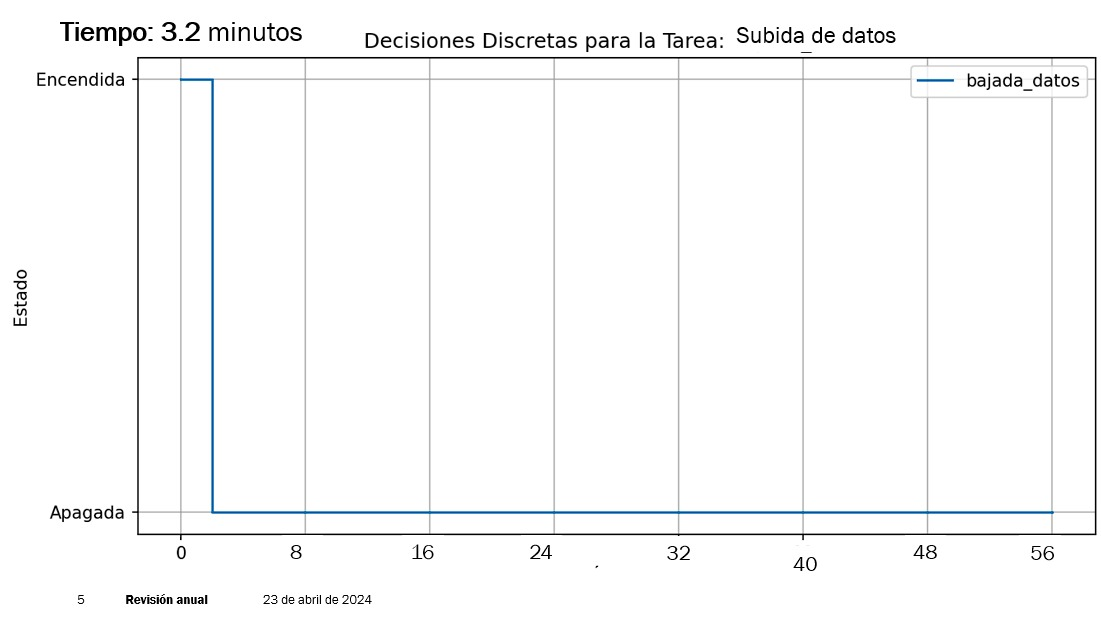
\includegraphics[width=0.9\textwidth]{subida-de-datos.jpeg}}
\end{frame}

\section{State of Charge}
\begin{frame}
  \frametitle{SoC}
  \centering
  \href{https://github.com/EnigmaK9/linx/tree/main/06-progress_04_22_2024/padilla-villanueva/sql}{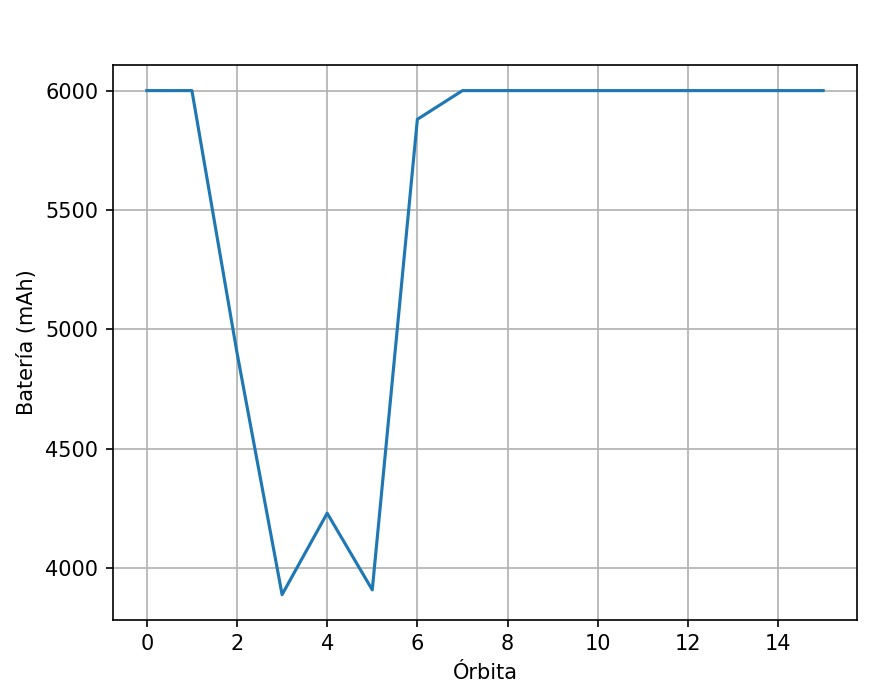
\includegraphics[width=0.9\textwidth]{bateria-orbita.jpeg}}
\end{frame}

\section{Design}
\begin{frame}
  \frametitle{Design}
  \centering
  \href{https://github.com/EnigmaK9/linx/tree/main/06-progress_04_22_2024/padilla-villanueva/sql}{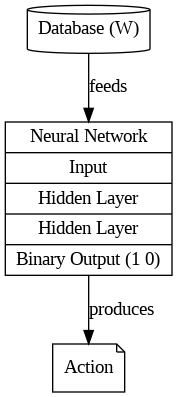
\includegraphics[width=0.2\textwidth]{descarga.png}}
\end{frame}



\section{Reward function's schema}
\begin{frame}{Reward function's schema}
  \href{https://colab.research.google.com/drive/1hqRPRc5jw_YP3mABA8Y5R_F7r0MRvMcT?usp=sharing}{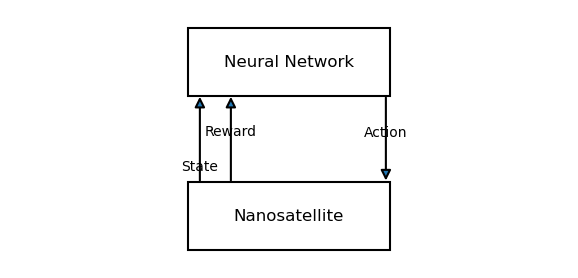
\includegraphics[width=0.9\textwidth]{reward.png}}

\end{frame}

\end{document}
